% --------------------------------------
% Document Class
% --------------------------------------
\documentclass[a4paper,11pt]{article}
% --------------------------------------



% --------------------------------------
% Use Package
% --------------------------------------


\usepackage[francais]{babel}
\usepackage{ucs}
\usepackage[utf8]{inputenc}
\usepackage[T1]{fontenc}

\usepackage{makeidx}
\usepackage{color}
\usepackage{graphicx}
\usepackage{float}
\usepackage[hidelinks]{hyperref} 
\usepackage{geometry}
%\usepackage{lastpage}
%\usepackage{marginnote}
\usepackage{fancyhdr}
%\usepackage{titlesec}
%\usepackage{framed}
\usepackage{amsmath}
\usepackage{empheq}
\usepackage{array}
\usepackage{multicol}
\usepackage{csquotes}
%\usepackage{adjustbox}

% insert code
\usepackage{listings}

% define our color
\usepackage{xcolor}

% code color
\definecolor{ligthyellow}{RGB}{250,247,220}
\definecolor{darkblue}{RGB}{5,10,85}
\definecolor{ligthblue}{RGB}{1,147,128}
\definecolor{darkgreen}{RGB}{8,120,51}
\definecolor{darkred}{RGB}{160,0,0}

% other color
\definecolor{ivi}{RGB}{141,107,185}

\def\verticaltext#1{\rotatebox[origin=c]{90}{\x{#1}}}


\lstset{
    language=python,
    captionpos=b,
    extendedchars=true,
    frame=lines,
    numbers=left,
    numberstyle=\tiny,
    numbersep=5pt,
    keepspaces=true,
    breaklines=true,
    showspaces=false,
    showstringspaces=false,
    breakatwhitespace=false,
    stepnumber=1,
    showtabs=false,
    tabsize=3,
    basicstyle=\small\ttfamily,
    backgroundcolor=\color{ligthyellow},
    keywordstyle=\color{ligthblue},
    morekeywords={include, printf, uchar},
    identifierstyle=\color{darkblue},
    commentstyle=\color{darkgreen},
    stringstyle=\color{darkred},
}


% --------------------------------------



% --------------------------------------
% Page setting
% --------------------------------------
%\pagestyle{empty}
\setlength{\headheight}{15pt}

\setcounter{secnumdepth}{3}
\setcounter{tocdepth}{2}

\makeatletter
\@addtoreset{chapter}{part}
\makeatother 

\hypersetup{       % parametrage des hyperliens
  colorlinks=true,  % colorise les liens
  breaklinks=true,  % permet les retours à la ligne pour les liens 
                    % trop longs
  urlcolor= blue,   % couleur des hyperliens
  linkcolor= black, % couleur des liens internes aux documents 
                    % (index, figures, tableaux, equations,...)
  citecolor= green  % couleur des liens vers les references 
                    % bibliographiques
}

% --------------------------------------

% --------------------------------------
% Information
% --------------------------------------
\title{
  \noindent\hrulefill \\
  \vspace{10mm}
  \textbf{Compte-rendu VisA} \\
  \vspace{5mm}
  TP: Approche de la logique floue.
}

\author{Gaëtan DEFLANDRE}
% --------------------------------------

\definecolor{myColor}{rgb}{0.5, 0.1, 0.75}

% --------------------------------------
% Begin content
% --------------------------------------
\begin{document}

\maketitle
\noindent\hrulefill \\


\section*{Introduction}

\newpage


\section{Fonctions d'appartenance}

\begin{figure}[H]
  \begin{center}
  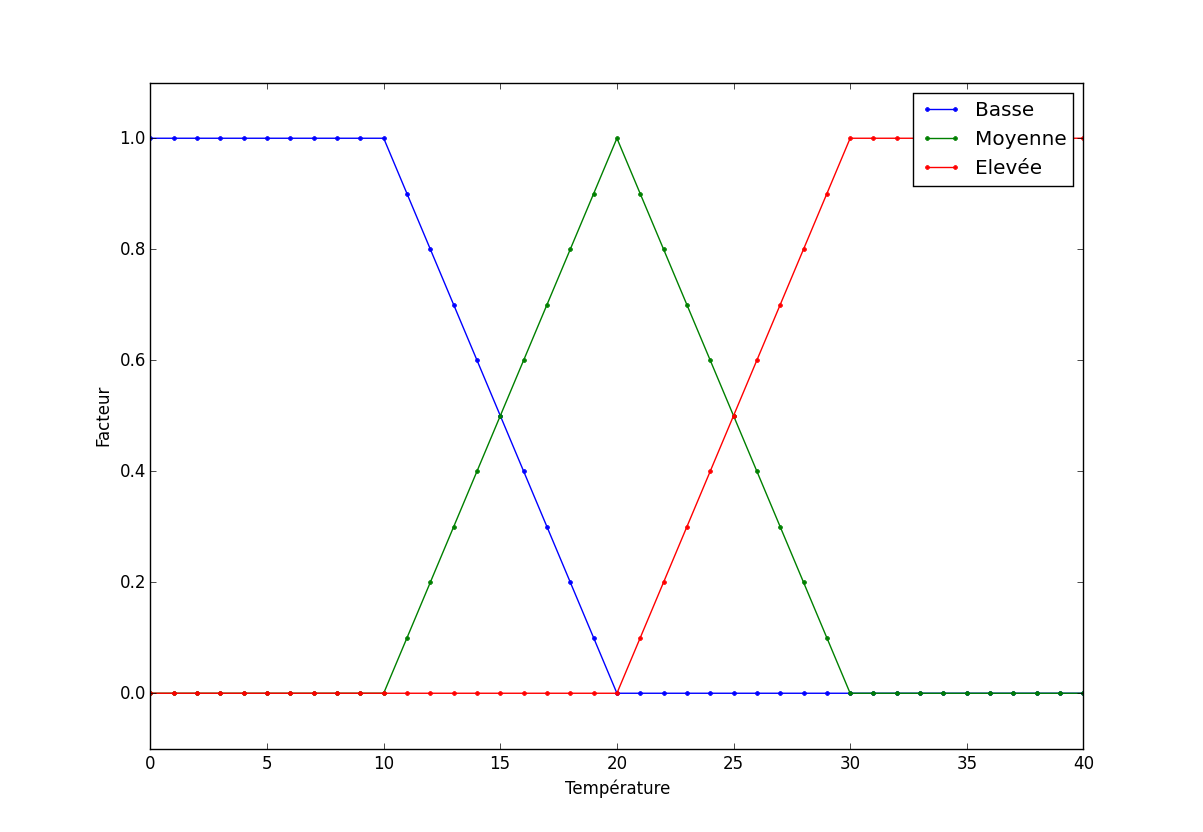
\includegraphics[height=280px]{images/exercice1.png}
  \caption{Les fonctions d'appartenance.}
  \end{center}
\end{figure}




\section{Opérateurs de la logique floue}

\begin{figure}[H]
  \begin{center}
  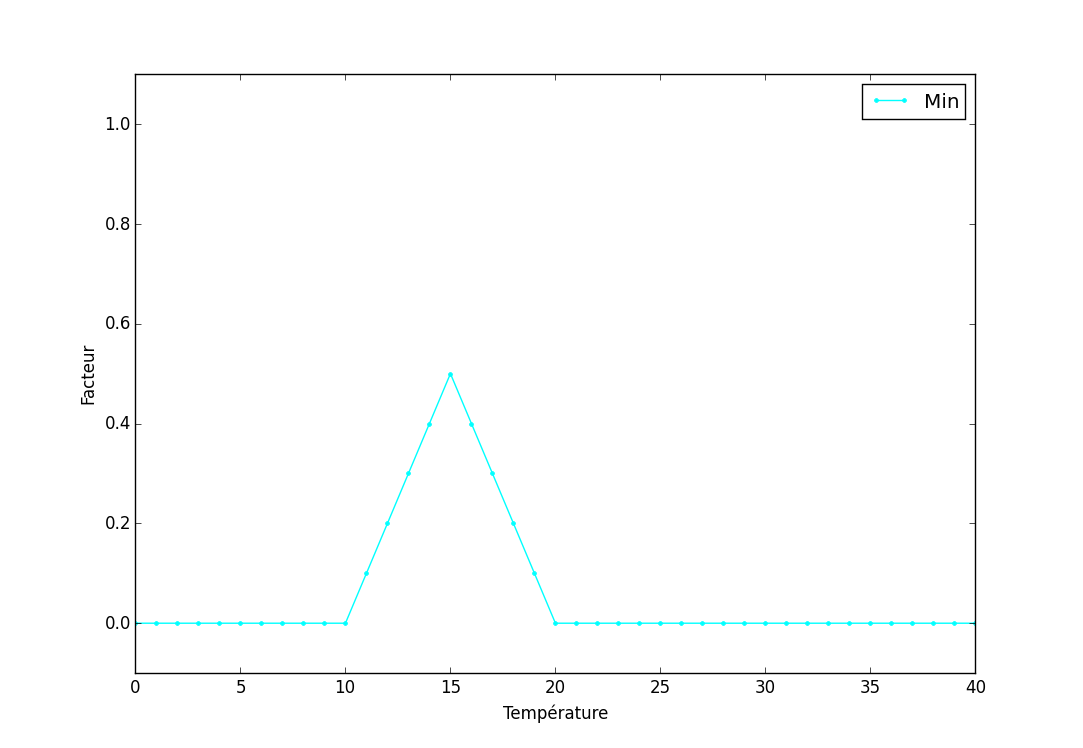
\includegraphics[height=280px]{images/min.png}
  \caption{Fonction minimum entre la fonction de température basse et moyenne.}
  \end{center}
\end{figure}



\begin{figure}[H]
  \begin{center}
  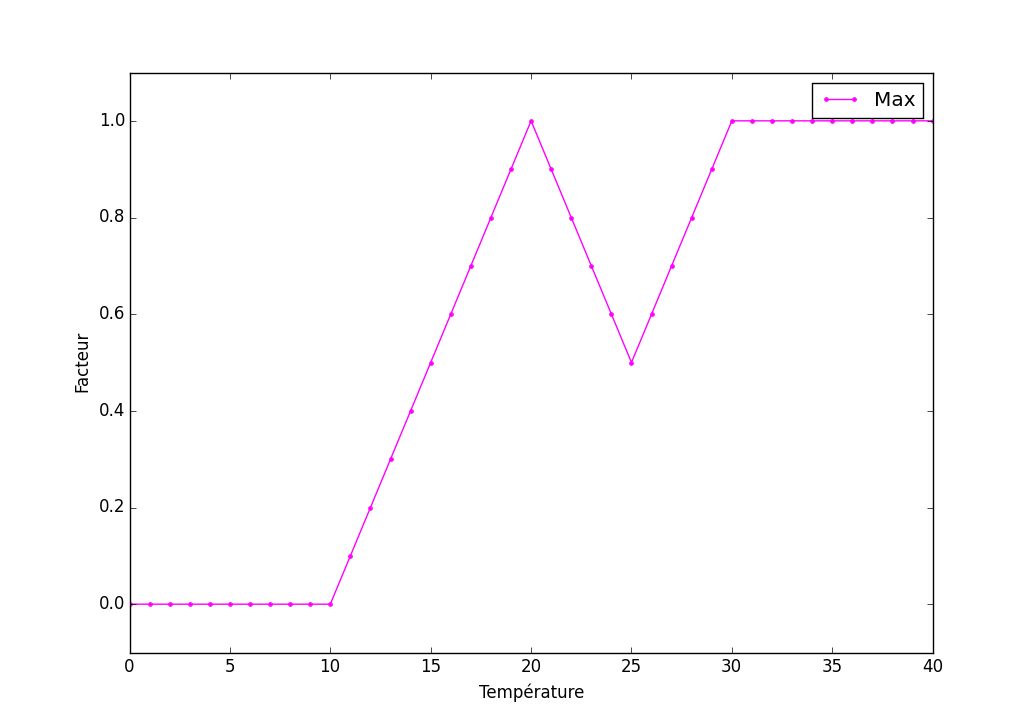
\includegraphics[height=280px]{images/max.png}
  \caption{Fonction maximum entre la fonction de température moyenne et haute.}
  \end{center}
\end{figure}




\section{Implication floue}

\begin{figure}[H]
  \begin{center}
  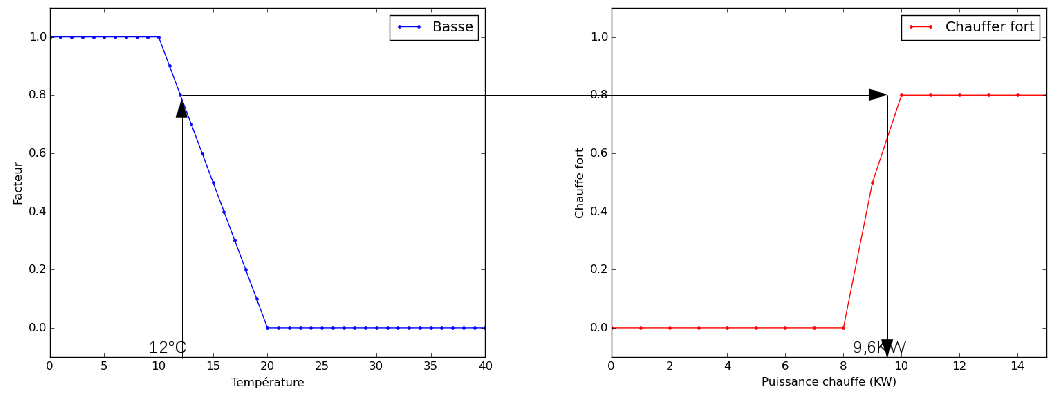
\includegraphics[height=170px]{images/low_mamdani_arrow.png}
  \caption{Fonction de température basse et implication floue.}
  \end{center}
\end{figure}




\section*{Conclusion}

\newpage





\section*{Conclusion}


\end{document}
